\documentclass[11pt,a4paper]{article}
\usepackage[margin=2.3cm]{geometry}
\usepackage[T1]{fontenc}
\usepackage{lmodern,microtype}
\usepackage{amsmath,amssymb,amsthm,bm}
\usepackage{booktabs,multirow,array,siunitx}
\usepackage{graphicx,subcaption}
\usepackage[ruled,vlined,linesnumbered]{algorithm2e}
\usepackage[numbers,sort&compress]{natbib}
\usepackage{xcolor}
\usepackage[gen]{eurosym}
\usepackage[colorlinks=true,linkcolor=blue!50!black,citecolor=blue!50!black,urlcolor=blue!50!black]{hyperref}
\usepackage[capitalise,noabbrev]{cleveref}
\sisetup{group-separator={,},group-minimum-digits=4}
\newtheorem{proposition}{Proposition}
\newcommand{\R}{\mathbb{R}}
\newcommand{\Z}{\mathbb{Z}}
\newcommand{\todo}[1]{\textcolor{red!70!black}{[TODO: #1]}}
\newcommand{\Egreedygap}{27.8}
\newcommand{\EoneTPcert}{0.81}
\newcommand{\EoneFullSec}{541}
\newcommand{\EoneFullGap}{0.01}
\newcommand{\EoneOpt}{11,532}
\newcommand{\LegacyReported}{729}
\newcommand{\LegacyTrue}{16,511}
\newcommand{\LegacyFactor}{23}
\newcommand{\EoneTPgap}{0.06}
\newcommand{\EoneTPsec}{9}
\newcommand{\EoneSavingPct}{30}
\newcommand{\AblText}{The inequalities raise the root LP bound by 14\% and 21\% on the two instances, but within 120\,s HiGHS's own cutting planes and branching make the final bounds of both variants comparable, and the full MILP does not converge faster. Their practical value is different: (SLOT) is required for the aggregated solution to be split into individual vehicles, and without it phase 1 can return plans that no fleet can execute. \Cref{tab:ablation} also shows that relaxing container integrality (phase 1) is what makes the problem easy: the relaxed model solves to optimality in seconds, whereas the integer one does not close in 120\,s.}
\newcommand{\ScalText}{On instances with fewer than 4,000 columns (12 instances) the two-phase scheme is the method of choice: mean gap 3.3\% to the lower bound in 31\,s on average, versus 8.8\% for ALNS started from the greedy plan (60\,s) and 35.6\% for the greedy rule, whose gap is inflated by stock it fails to place within capacities and fleet days. ALNS polishing improves the two-phase plans only marginally (by less than 0.01\%) on these sizes. The picture reverses on the largest class (about 8,100 columns): phase~1 does not converge within its 60\,s budget, its incumbent leaves 114--128\,t unshipped and the restricted phase~2 cannot recover; ALNS from the greedy plan is then the best method (mean gap 21.8\% against the relaxation bound, versus 36.6\% for greedy). The two methods are therefore complementary, and seeding phase~2 with ALNS or greedy routes is an obvious improvement. All gaps are measured against relaxation bounds and overstate the true sub-optimality: on the case study the phase-1 bound was 0.8\% below the proven optimum.}
\newcommand{\SensText}{Internalising a carbon price of 500\,\euro/t cuts emissions from 4.85 to 4.45\,t (8\%) at a cost increase of 0.9\% (\cref{fig:sens}). Scaling the monthly volume from 0.5$\times$ to 3$\times$ moves the cost per tonne from 153 to 701\,\euro{} and the share treated in Spain from 67\% to 44\%, as Spanish capacity saturates; at 3$\times$ the volume 30\,t (lead--acid) cannot be placed within contracted capacities at all, which is precisely the situation the strategic model of \cref{sec:strategic} is designed to anticipate.}
\newcommand{\VSSpct}{6.5}
\newcommand{\StratText}{The stochastic design invests more up front than the expected-value design (22.8 vs 8.5\,M\euro{} of discounted depot and plant costs) and recovers it in operation: second-stage costs fall by 3.2, 7.8 and 54.4\,M\euro{} in the pessimistic, neutral and optimistic scenarios. The expected-value design (Madrid + Bilbao depots; only Leon plant in 2035) leaves 28.1\,kt of Li-ion untreated over the horizon if adoption is fast, versus 2.5\,kt for the stochastic design. EVPI is 12.4\% of the expected cost, an upper bound on what better demand forecasts are worth. Across $P(\text{optimistic})\in\{0.1,0.25,0.4\}$ and plant-cost multipliers $\{0.75,1,1.5\}$, the first Spanish Li-ion plant opens between 2032 and 2034, except when the optimistic scenario is unlikely ($p=0.1$) and plants are not cheaper than assumed ($\times$1, $\times$1.5), in which case none is built.}
\newcommand{\FirstMileText}{On the uniform benchmark, CW+LS is within a few percent of the best-known values reported in the learning-to-route literature (about 6.1, 10.4 and 15.7 for $n=20,50,100$ \citep{kool2019,kwon2020}). \todo{Train POMO on a GPU (\texttt{python -m brlo.firstmile.train}) and add its results; the published POMO numbers suggest gaps of about 1\% to optimal on uniform instances.}}


\title{\textbf{A hierarchical optimisation framework for the reverse logistics of end-of-life EV batteries:}\\[2pt]
stochastic network design, certified long-haul dispatch and learned first-mile collection}
\author{Miguel Lozano Nykolaychuk\\{\small Universidad Carlos III de Madrid}}
\date{\small Preprint -- \today}

\begin{document}
\maketitle

\begin{abstract}
The growth of electric mobility will turn end-of-life (EOL) traction batteries into one of the fastest-growing hazardous waste streams in Europe, and the cost and carbon footprint of moving them to recyclers are decisive for the viability of a circular battery economy. Taking as a case study a Spanish battery take-back scheme that ships sorted waste from a storage depot near Madrid to recyclers in France and Germany, we propose a three-level decision framework.
(i) At the strategic level, a two-stage stochastic multi-period network design model decides which storage depots to operate and whether and when to build treatment capacity in Spain under pessimistic, neutral and optimistic EV-adoption scenarios; on our illustrative data the stochastic solution is worth \VSSpct\% of expected cost relative to planning with the mean scenario.
(ii) At the operational long-haul level, a set-partitioning mixed-integer programme with a heterogeneous (diesel and battery-electric) fleet, multiple waste streams, split deliveries, homologated containers, load-dependent fuel and CO$_2$, and EU Regulation 561/2006 driving times is solved by a two-phase scheme that \emph{certifies} its own optimality gap; on the case study it returns in \EoneTPsec\,s a plan certified within \EoneTPcert\% and actually within \EoneTPgap\% of the optimum, which the full MILP proves in \EoneFullSec\,s. An ALNS matheuristic complements it for larger instances.
(iii) For first-mile collection from workshops and dealers, an attention-based constructive policy trained with reinforcement learning (POMO) is benchmarked against Clarke--Wright savings with local search.
An audit of the ERP prototype that originally addressed the problem shows that it under-reported the cost of its own plan by a factor of \LegacyFactor{} and produced overloaded vehicles; the certified plan is \EoneSavingPct\% cheaper than the legacy plan's true cost. All code is open source.
\end{abstract}

\noindent\textbf{Keywords:} reverse logistics; battery recycling; stochastic programming; vehicle routing; matheuristics; neural combinatorial optimisation; reinforcement learning.

% =====================================================================
\section{Introduction}
\label{sec:intro}
Battery-electric vehicles shift the environmental burden of road transport from the tailpipe to the battery supply chain. Recovering lithium, nickel, cobalt and manganese from EOL batteries reduces the need for primary extraction and is now mandated in the European Union by Regulation (EU) 2023/1542, which sets collection targets, minimum recycling efficiencies, material-recovery levels and recycled-content requirements for new batteries \citep{EUbattery2023}. Recycling technology itself is maturing \citep{harper2019}, but the logistics around it are expensive: EOL batteries are dangerous goods (UN~3480/3090 or class~8 for lead--acid) that travel in certified, heavy containers, and recycling capacity is concentrated in a few plants, often far from where batteries are collected.

This paper revisits and substantially extends a bachelor thesis \citep{lozano2024} that studied the supply chain of Ecopilas, the largest battery take-back scheme in Spain. In 2024 the scheme sent its sorted waste from a temporary storage depot to two recyclers, SNAM (France) and ACCUREC (Germany), $\sim$1{,}200--1{,}800\,km away, while several Spanish facilities were emerging. The thesis delivered a prototype inside a commercial ERP (Microsoft Dynamics 365 Business Central) that selected recyclers and trucks with a greedy rule. Here we replace it with an open-source framework with a solid theoretical basis and answer three questions at three planning levels:
\begin{enumerate}
\item \textbf{Strategic} (years): given uncertain growth in EOL volumes, which depots should operate, and should treatment capacity be built in Spain instead of shipping abroad -- and when? (\cref{sec:strategic})
\item \textbf{Long-haul dispatch} (weeks--months): given stocks at the depots, which facility should receive each stream, with which vehicles, on which multi-stop trips? (\cref{sec:longhaul})
\item \textbf{First-mile collection} (days): how should collectors route through hundreds of workshops and dealers every day? (\cref{sec:firstmile})
\end{enumerate}

\paragraph{Contributions.}
\begin{itemize}
\item A set-partitioning formulation of multi-stream long-haul dispatch in which \emph{load-dependent} energy use and CO$_2$ are exactly linear, together with a schedule model of EU Regulation 561/2006 \citep{EU561} embedded in the route costs, valid inequalities, and a two-phase scheme that returns plans with a certified optimality gap (\cref{prop:lb}).
\item An ALNS matheuristic \citep{ropke2006,maniezzo2009} that searches route skeletons and evaluates each one exactly with the restricted MILP, for instances where the column pool cannot be enumerated.
\item A two-stage stochastic multi-period network design model fed by the same trip-cost model and by continuum approximations of collection tours \citep{beardwood1959,daganzo1984}, with the value of the stochastic solution (VSS) and of perfect information (EVPI) \citep{birge2011}.
\item A learned first-mile policy (attention model + POMO, \citep{kool2019,kwon2020}) in PyTorch, benchmarked on clustered instances that mimic the spatial structure of collection points.
\item A reproducible audit of the original ERP heuristic with the same independent evaluator, and an open-source Python package with tests (scipy/HiGHS \citep{huangfu2018,virtanen2020}, PyTorch \citep{paszke2019}); no commercial licence is required.
\end{itemize}

% =====================================================================
\section{Related work}
\label{sec:related}
\paragraph{Reverse logistics network design.} Quantitative reverse logistics was surveyed early by \citet{fleischmann1997}; \citet{govindan2015} review closed-loop supply chains and \citet{melo2009} the role of facility location. For EV batteries specifically, \citet{hoyer2015} plan technology and capacity of recycling in Germany. Uncertainty in return volumes motivates stochastic programming \citep{birge2011}; we follow the standard two-stage approach and report VSS/EVPI.
\paragraph{Routing.} Our long-haul problem combines a heterogeneous fleet \citep{koc2016}, split deliveries \citep{archetti2012}, load-dependent fuel use as in the pollution-routing problem \citep{bektas2011,xiao2012}, drivers' working-hour regulations \citep{goel2009}, and hazardous materials \citep{erkut2007}; facility selection links it to location-routing \citep{prodhon2014}. Set-partitioning formulations are classical in routing \citep{toth2014}. ALNS \citep{ropke2006} is the reference metaheuristic for rich VRPs.
\paragraph{Learning to route.} Pointer networks \citep{vinyals2015} and RL training \citep{bello2016,nazari2018} started neural combinatorial optimisation; the attention model of \citet{kool2019} and POMO \citep{kwon2020} are now standard constructive baselines; see \citet{bengio2021} for a methodological overview. State-of-the-art classical solvers such as HGS \citep{vidal2022,wouda2024} remain stronger on large instances; the appeal of learned policies is fast, amortised inference on recurring instances drawn from a fixed distribution -- exactly the daily first-mile setting.

% =====================================================================
\section{Audit of the original prototype}
\label{sec:audit}
The 2024 prototype \citep{lozano2024} processed each waste stream independently. ``Option~1'' sorted the recyclers that accept the stream by unit price, ``Option~2'' by \emph{ascending monthly capacity} (the thesis describes it as the shortest route, but distance is never used to rank or select facilities), and both filled facilities greedily and visited them in that order. We re-implemented it line by line (\texttt{brlo.longhaul.legacy}) and identified the following defects: (a) no consolidation across streams; (b) the return leg is not counted; (c) the gross vehicle weight was used as cargo capacity; (d) only one vehicle of each type can be used, so any remainder is silently dropped; (e) minimum lots and facility-wide capacities are ignored; (f) only fuel is costed (no driver time, tolls, rests); (g) container counts were computed with a cumulative-subtraction bug; (h) costs and maps used two different distance providers; and (i) an API key was embedded in the source code. \Cref{tab:case} prices the legacy plans with the independent evaluator of \cref{sec:eval}.

% =====================================================================
\section{Long-haul dispatch}
\label{sec:longhaul}
\subsection{Problem}
A set of depots $O$ hold stocks $s_{ok}$ of waste streams $k\in K$ (NMC/NCA and LFP traction packs, portable Li-ion, Ni-MH, Ni-Cd, lead--acid). Facilities $j\in J$ accept a subset $K_j$ of streams at gate fee $f_{jk}$ (negative when recovered metal value exceeds treatment cost), with contracted capacities $Q_{jk}$ and $Q_j$ and minimum lots $m_{jk}$. Each stream travels in its homologated container (net capacity $c_k$, tare $T_k$, floor slots $\sigma_k$). Vehicle types $v\in V$ (rigid 12\,t and 26\,t, 40\,t articulated, 19\,t battery-electric) have payload $P_v$, slots $S_v$, a daily range for electric trucks and $H_v$ available vehicle-days. Unshipped stock costs $\pi$ per kg. A trip leaves a depot, visits at most $L$ facilities and returns empty-handed (empty containers come back).

\subsection{Trip cost model}
For a trip of vehicle $v$ on legs $\ell=0,\dots,m$ of length $d_\ell$, energy per km is linear in the carried mass $W$: $e(W)=e_v^0+(e_v^1-e_v^0)W/P_v$ \citep{xiao2012,bektas2011}. Since $W_\ell$ equals the tare on board plus all deliveries made \emph{after} leg $\ell$,
\begin{equation}
\text{cost}=F_r+\sum_{\ell=0}^{m}\beta_\ell W_\ell,\qquad \beta_\ell=d_\ell\,\frac{e^1_v-e^0_v}{100P_v}\,(p_v+\lambda\,\epsilon_v),
\end{equation}
where $p_v$ is the energy price, $\epsilon_v$ the CO$_2$ intensity and $\lambda$ an optional carbon price. The fixed part $F_r$ adds a dispatch cost, a per-km cost (tolls, maintenance), zero-load energy, and paid driver time plus per-diems. Driver time comes from a simulation of Regulation 561/2006 for one driver: a 45-min break after 4.5\,h of driving, at most 9\,h of driving per day and an 11\,h daily rest, splitting legs when a limit is reached. A Madrid--Krefeld round trip, for instance, needs about five duty days.

\subsection{Set-partitioning formulation}
Let $R$ be the set of columns $r=(o,v,(j_{r1},\dots,j_{rm_r}))$ with $m_r\le L$; by default each facility subset keeps its distance-minimising order. Variables: $y_r\in\Z_+$ trips on column $r$; $x_{rik}\ge 0$ kg of $k$ delivered at stop $i$; $n_{rik}\in\Z_+$ containers; $z_{jk}\in\{0,1\}$; $u_{ok}\ge 0$. With $B_{ri}=\sum_{\ell\le i}\beta_{r\ell}$ and $B_r=\sum_\ell\beta_{r\ell}$:
\begin{align}
\min\ & \sum_r F_r y_r+\sum_{r,i,k}(f_{j_{ri}k}+B_{ri})x_{rik}+\sum_{r,i,k}T_kB_r n_{rik}+\pi\sum_{o,k}u_{ok} \label{eq:obj}\\
\text{s.t. } & \textstyle\sum_{r\in R_o}\sum_i x_{rik}+u_{ok}=s_{ok} && \forall o,k \label{eq:supply}\\
& m_{jk}z_{jk}\le \textstyle\sum_{(r,i):j_{ri}=j}x_{rik}\le Q_{jk}z_{jk},\quad \sum_k\sum_{(r,i):j_{ri}=j}x_{rik}\le Q_j && \forall j,k \label{eq:cap}\\
& x_{rik}\le c_k n_{rik} && \forall r,i,k \label{eq:pack}\\
& \textstyle\sum_{i,k}(x_{rik}+T_kn_{rik})\le P_v y_r,\quad \sum_{i,k}\sigma_k n_{rik}\le S_v y_r && \forall r \label{eq:payload}\\
& \textstyle\sum_{r:v(r)=v}\delta_r y_r\le H_v && \forall v \label{eq:fleet}
\end{align}
where $\delta_r$ is the number of calendar days of the trip. Because the $y_r$ identical trips of a column are aggregated, the plan is disaggregated into individual vehicles by first-fit decreasing, with an exact assignment MILP as fallback; the evaluator then audits it.

\paragraph{Valid inequalities.} (VUB) $x_{rik}\le U_{rik}y_r$ with $U_{rik}=\min\{s_{ok},Q_{jk},Q_j,P_v-T_k\}$, and the per-stop analogue; (SLOT) $\sum_{i,k:\sigma_k=\sigma}n_{rik}\le\lfloor S_v/\sigma\rfloor y_r$, which removes aggregated solutions that cannot be split into trucks (e.g.\ 33 two-slot boxes in two 33-slot trailers). \Cref{tab:ablation} reports their effect.

\begin{proposition}\label{prop:lb}
Let $z^{\mathrm{rel}}$ be the optimal value (or any dual bound) of \eqref{eq:obj}--\eqref{eq:fleet} with $n_{rik}\in\R_+$. Then $z^{\mathrm{rel}}\le z^\star$. If $\hat R\subseteq R$ and $\hat y$ bounds are imposed, the optimum of the restricted model is feasible for the full model, hence an upper bound.
\end{proposition}
\begin{proof}
Relaxing integrality enlarges the feasible set; restricting columns shrinks it.
\end{proof}
\noindent The \emph{two-phase scheme} solves the relaxation (phase 1, a lower bound), then re-solves the integer model on the columns used in phase 1, the same stop sets with every vehicle type, and their subsets, each with one extra trip allowed (phase 2, an upper bound), and reports the certified gap $(\mathrm{UB}-\mathrm{LB})/\mathrm{UB}$.

\subsection{ALNS matheuristic}
For large instances the column pool grows as $O(|O||V|\sum_{\ell\le L}\binom{|J|}{\ell})$. The matheuristic (\cref{alg:alns}) searches a small multiset of trip templates; each candidate is evaluated \emph{exactly} by the MILP restricted to it, which decides loads, containers, facility use and how many of the allowed trips to run. Destroy operators: random, worst-utilisation and facility removal; repair: direct template, cheapest insertion, merge, vehicle change, extra trip. Acceptance follows simulated annealing and operator weights are adapted as in \citet{ropke2006}.

\begin{algorithm}[t]
\caption{ALNS over route skeletons with exact MILP evaluation}\label{alg:alns}
\KwIn{initial plan (greedy or two-phase)}
$\mathcal S\gets$ templates of the initial plan; $(c,\cdot)\gets\mathrm{MILP}(\mathcal S)$; $\mathcal S^\star\gets\mathcal S$\;
\While{time and iterations remain}{
 choose destroy $d$ and repair $\rho$ by roulette on weights\;
 $\mathcal S'\gets\rho(d(\mathcal S))$\;
 $(c',\text{used})\gets\mathrm{MILP}(\mathcal S')$ \tcp*{memoised}
 \lIf{$c'<c^\star$}{$\mathcal S^\star\gets\mathcal S'$}
 \lIf{$c'<c$ \textbf{or} $\mathrm{rand}<e^{-(c'-c)/T}$}{$\mathcal S\gets$ used part of $\mathcal S'$}
 update scores; $T\gets 0.995\,T$; every 50 iterations update weights\;
}
\Return plan of $\mathcal S^\star$
\end{algorithm}

\subsection{Independent evaluation}\label{sec:eval}
Every method outputs a list of trips, which a common evaluator re-prices from scratch and checks 14 types of violation (payload, slots, container capacity, compatibility, facility capacities, minimum lots, stock balance, fleet days, electric range, maximum stops, segregation). All numbers reported below come from this evaluator.

% =====================================================================
\section{Strategic network design}
\label{sec:strategic}
Regions $i$ (15 peninsular NUTS-2 regions, weighted by population) generate EOL tonnes $D_{ikts}$ of chemistry groups $k\in\{\text{Li},\text{Ni},\text{Pb}\}$ in years $t$ under scenarios $s$ with probabilities $p_s$. First-stage binaries $a_{dt}$ (depot $d$ operates) and $b_{jt}$ (candidate plant $j$ operates, monotone, subject to a construction lead time) are fixed before uncertainty resolves; flows $f_{idkts}$, $g_{djkts}$ and shortfalls $u_{ikts}$ are recourse:
\begin{align}
\min\ &\sum_t\delta^t\Big[\sum_d F^D_d a_{dt}+\sum_j F^P_j b_{jt}\Big]+\sum_s p_s\sum_t\delta^t\Big[\sum c^1_{id}f_{idkts}+\sum(c^2_{dj}+\phi_{jk})g_{djkts}+\pi\sum u_{ikts}\Big]\\
\text{s.t. }&\textstyle\sum_d f_{idkts}+u_{ikts}=D_{ikts},\quad \sum_i f_{idkts}=\sum_j g_{djkts},\quad \sum_{i,k}f_{idkts}\le K_d a_{dt},\\
&\textstyle\sum_d g_{djkts}\le Q_{jk}b_{jt},\quad a_{dt}\ge a_{d,t-1},\ b_{jt}\ge b_{j,t-1}.
\end{align}
Depot-to-plant rates $c^2_{dj}$ (\euro/t) are computed with the trip-cost model of \cref{sec:longhaul} for a full 40\,t truck at 85\% load, so that both levels price transport consistently. Region-to-depot rates add a line-haul term and a local collection term from the continuum approximation $L\approx 2\bar r N/C+k\sqrt{NA}$ \citep{beardwood1959,daganzo1984}. We compute the recourse problem (RP), the expected-value problem (EV) and the expected result of using its design (EEV), and the wait-and-see value (WS); $\mathrm{VSS}=\mathrm{EEV}-\mathrm{RP}$ and $\mathrm{EVPI}=\mathrm{RP}-\mathrm{WS}$ \citep{birge2011}.

% =====================================================================
\section{Learned first-mile collection}
\label{sec:firstmile}
Collection from workshops, dealers and dismantlers to a regional depot is a capacitated VRP that recurs daily with similar spatial structure. We train an attention policy \citep{kool2019} with POMO \citep{kwon2020}: an encoder of six transformer layers ($d=128$, eight heads, instance normalisation) embeds the depot and customers $(x,y,q/Q)$; at each step the decoder queries with the last node embedding and the remaining load, performs a multi-head glimpse and outputs masked, tanh-clipped logits. For an instance with $n$ customers, $n$ rollouts start from different first customers and share the baseline $b=\frac1n\sum_p L_p$; the REINFORCE gradient is $\nabla_\theta J\approx\frac{1}{Bn}\sum_{b,p}(b_b-L_{bp})\nabla_\theta\log\pi_\theta(\tau_{bp})$. Inference decodes all starts greedily on the eight symmetries of the unit square. Besides the uniform benchmark distribution \citep{nazari2018,kool2019} we train on a \emph{clustered} distribution (Gaussian town clusters plus a rural background, an off-centre depot, frequent light pick-ups of portable batteries and rarer heavy EV modules).

% =====================================================================
\section{Computational study}
\label{sec:results}
All experiments ran on a 2-core cloud CPU with HiGHS through \texttt{scipy.optimize.milp}. Locations of the case study are city-level coordinates of the facilities named in \citep{lozano2024}; road distance is great circle $\times$ 1.25 \citep{ballou2002}, which reproduces the 1{,}780\,km Madrid--Krefeld route of the thesis within 3\%. \textbf{Gate fees, contracted capacities and stocks are synthetic} (the companies did not disclose them) but plausible; all values are in \texttt{brlo/data/instances.py}.

\subsection{Case study: one month of the Madrid depot}
\begin{table}[t]\centering\small\setlength{\tabcolsep}{4pt}
\caption{Case study (one month, 71\,t). Costs in \euro{{}} recomputed by the independent evaluator; `reported' is what the legacy prototype displayed; gap is relative to the best lower bound (11,532\,\euro).}\label{tab:case}
\begin{tabular}{lrrrrrrlrr}\toprule
Method & Reported & Cost & Transport & Fees & CO$_2$ (t) & Trips & Feasible & Gap \% & s\\\midrule
Legacy BC prototype, option 1 & 729 & 16,511 & 20,281 & -3,770 & 12.17 & 6 & no (5) & -- & 0.0\\
Legacy BC prototype, option 2 & 16,707 & 25,822 & 15,122 & 10,700 & 8.96 & 6 & no (9) & -- & 0.0\\
Greedy (corrected) & -- & 15,978 & 19,373 & -3,395 & 11.81 & 6 & yes & 27.83 & 0.0\\
ALNS from greedy (120 s) & -- & 11,984 & 9,234 & 2,750 & 5.41 & 5 & yes & 3.78 & 19.6\\
Two-phase MILP (certified) & -- & 11,538 & 8,533 & 3,005 & 4.85 & 6 & yes & 0.06 & 8.6\\
Full MILP (600 s) & -- & 11,533 & 8,528 & 3,005 & 4.92 & 5 & yes & 0.01 & 540.7\\
\bottomrule\end{tabular}\end{table}

\Cref{tab:case} compares methods on 71\,t of mixed battery waste. The legacy prototype reports \LegacyReported\,\euro{} for its Option~1 plan, which actually costs \LegacyTrue\,\euro{} and overloads vehicles. The corrected greedy rule is feasible but \Egreedygap\% above the optimum; ALNS started from it closes most of that gap. The two-phase scheme returns in \EoneTPsec\,s a plan with a certified gap of \EoneTPcert\%; the full MILP with integer containers proves the optimum (\EoneOpt\,\euro{}, residual gap \EoneFullGap\%) only after \EoneFullSec\,s, which shows that the two-phase plan was within \EoneTPgap\% of optimal. \Cref{fig:map} shows the certified plan: lead--acid and Ni streams consolidate towards Bizkaia, most cobalt-rich NMC goes to France, where the fee is negative, and LFP and second-life streams are served by Spanish facilities on multi-stop trips.

\begin{figure}[t]\centering
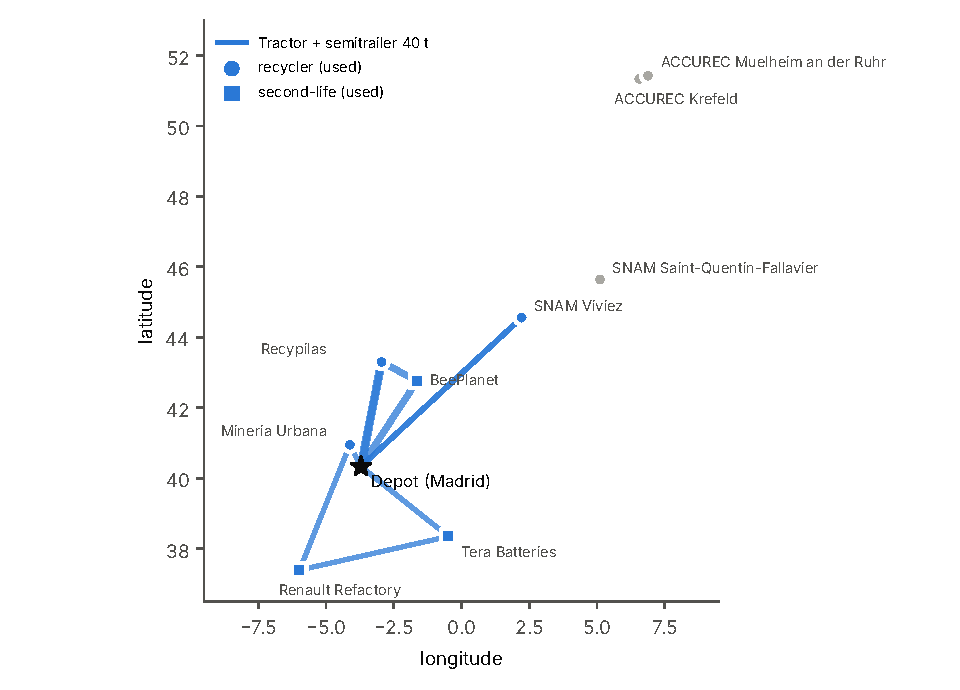
\includegraphics[width=0.85\linewidth]{figures/case_network.pdf}
\caption{Certified long-haul plan for the case study (straight segments; line width proportional to cargo).}\label{fig:map}
\end{figure}

\subsection{Ablation of the formulation}
\begin{table}[t]\centering\small
\caption{Effect of the valid inequalities (VUB+SLOT): LP root bound, optimum with continuous containers (phase 1), and bound/incumbent of the full MILP after 120\,s.}\label{tab:ablation}
\begin{tabular}{lcrrrrr}\toprule
Instance & Ineq. & LP root & Phase-1 opt. & Full LB & Full UB & s\\\midrule
iberia\_base & no & 9,547 & 11,444 & 11,301 & 11,563 & 120\\
iberia\_base & yes & 10,880 & 11,444 & 11,097 & 11,809 & 120\\
rand\_f12\_s0 & no & 6,541 & 8,825 & 8,379 & 9,328 & 120\\
rand\_f12\_s0 & yes & 7,921 & 8,825 & 8,362 & 9,474 & 120\\
\bottomrule\end{tabular}\end{table}

\AblText

\subsection{Scalability}
\begin{table}[t]\centering\small\setlength{\tabcolsep}{4pt}
\caption{Random instances (mean over seeds): gap (\%) to the phase-1 lower bound and seconds.}\label{tab:scal}
\begin{tabular}{rrrrrrrrrrr}\toprule
$|J|$ & $|O|$ & columns & \multicolumn{2}{c}{Greedy} & \multicolumn{2}{c}{ALNS} & \multicolumn{2}{c}{Two-phase} & \multicolumn{2}{c}{Two-phase+ALNS}\\
 & & & gap & s & gap & s & gap & s & gap & s\\\midrule
8 & 1 & 276 & 36.30 & 0 & 4.48 & 60 & 1.28 & 19 & 1.28 & 65\\
12 & 1 & 895 & 51.86 & 0 & 7.42 & 60 & 1.60 & 13 & 1.60 & 58\\
12 & 2 & 1,793 & 22.17 & 0 & 15.72 & 60 & 8.12 & 74 & 8.12 & 120\\
16 & 1 & 2,090 & 31.87 & 0 & 7.68 & 60 & 2.08 & 20 & 2.08 & 65\\
20 & 2 & 8,110 & 36.64 & 0 & 21.76 & 61 & 94.56 & 149 & 58.88 & 194\\
\bottomrule\end{tabular}\end{table}

\ScalText
\begin{figure}[t]\centering
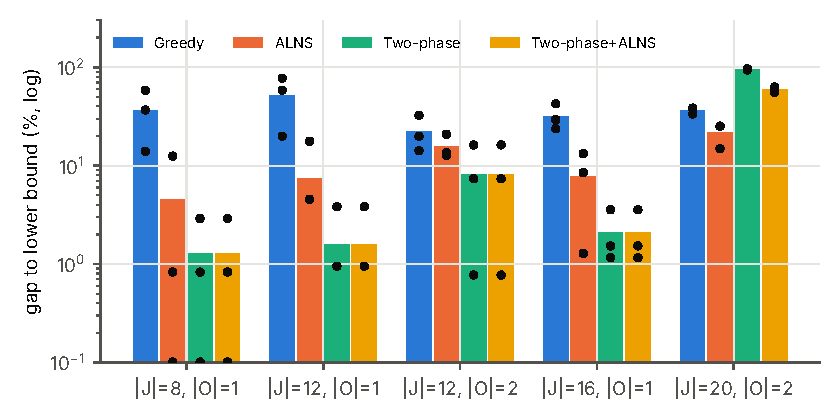
\includegraphics[width=0.75\linewidth]{figures/scalability.pdf}
\caption{Gap to the lower bound (phase-1 relaxation) by method and instance size; dots are instances, bars the mean.}\label{fig:scal}
\end{figure}

\subsection{Carbon price and volume sensitivity}
\begin{figure}[t]\centering
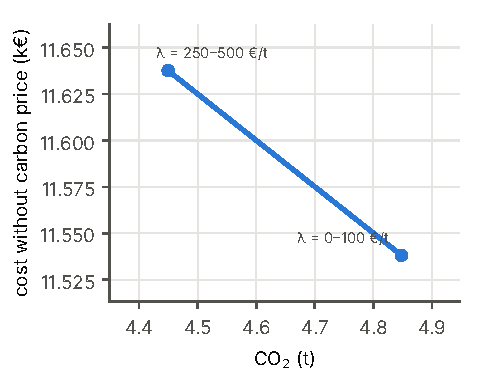
\includegraphics[width=0.48\linewidth]{figures/co2_tradeoff.pdf}\hfill
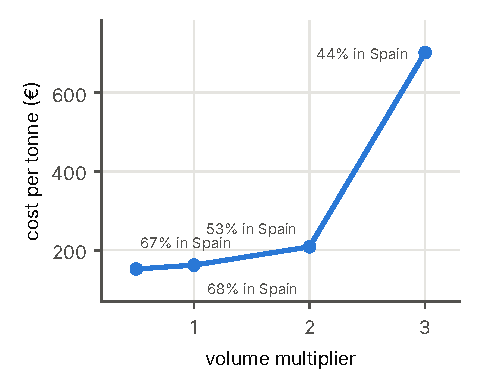
\includegraphics[width=0.48\linewidth]{figures/volume_scale.pdf}
\caption{Left: cost--CO$_2$ trade-off when a carbon price $\lambda$ is internalised. Right: cost per tonne and share treated in Spain when the monthly volume is scaled.}\label{fig:sens}
\end{figure}
\SensText

\subsection{Strategic design under uncertainty}
\begin{table}[t]\centering\small
\caption{Stochastic network design, 2026--2035 (discounted M\euro). Designs list the first operating year of each additional depot and new plant.}\label{tab:strategic}
\begin{tabular}{lr}\toprule Measure & M\euro\\\midrule
RP & 61.87\\
EV & 53.61\\
EEV & 65.88\\
WS & 54.20\\
VSS = EEV $-$ RP & 4.02 (6.5\%)\\
EVPI = RP $-$ WS & 7.67 (12.4\%)\\
\bottomrule\end{tabular}\\[6pt]
\begin{tabular}{ll}\toprule Model & Design\\\midrule
RP & depots: BIO~2026, ZAZ~2033; plants: LEON~2035, ZAZ~2033\\
EV & depots: BIO~2026; plants: LEON~2035\\
WS pessimistic & depots: BIO~2026; plants: none\\
WS neutral & depots: BIO~2026; plants: none\\
WS optimistic & depots: BIO~2026, ZAZ~2034; plants: LEON~2032, ZAZ~2034\\
\bottomrule\end{tabular}\end{table}

\begin{figure}[t]\centering
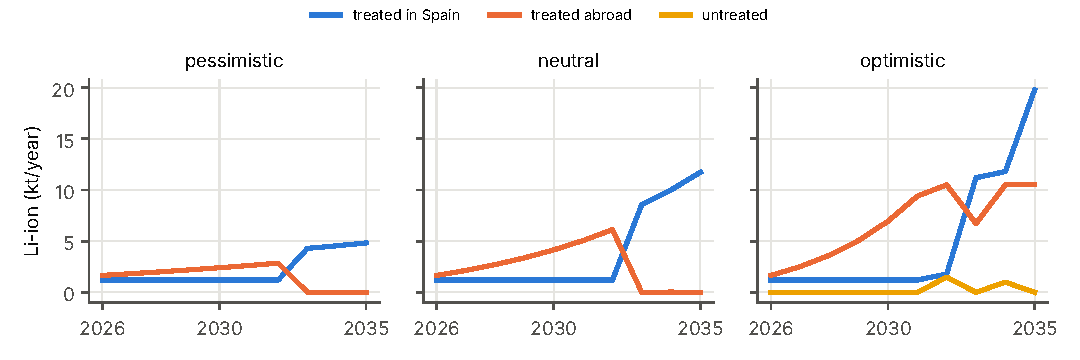
\includegraphics[width=\linewidth]{figures/strategic_flows.pdf}
\caption{Li-ion tonnes treated in Spain and abroad per year in the stochastic (RP) design, by scenario.}\label{fig:flows}
\end{figure}
\StratText

\subsection{First-mile collection}
\begin{table}[t]\centering\small\setlength{\tabcolsep}{4pt}
\caption{First-mile CVRP, mean tour length on 100 test instances (unit square; gaps relative to CW+LS).}\label{tab:firstmile}
\begin{tabular}{lrllll}\toprule Distribution & $n$ & Nearest neighbour & Clarke--Wright & CW + local search & POMO ($\times$8 aug.)\\\midrule
clustered & 20 & 4.426 (+25.4\%) & 3.569 (+1.1\%) & 3.529 (1\,ms) & \todo{GPU run}\\
clustered & 50 & 7.704 (+24.2\%) & 6.314 (+1.8\%) & 6.204 (4\,ms) & \todo{GPU run}\\
clustered & 100 & 11.218 (+21.8\%) & 9.357 (+1.6\%) & 9.209 (19\,ms) & \todo{GPU run}\\
uniform & 20 & 7.933 (+28.0\%) & 6.244 (+0.7\%) & 6.200 (1\,ms) & \todo{GPU run}\\
uniform & 50 & 13.958 (+31.1\%) & 10.745 (+1.0\%) & 10.643 (5\,ms) & \todo{GPU run}\\
uniform & 100 & 21.254 (+28.0\%) & 16.760 (+0.9\%) & 16.607 (15\,ms) & \todo{GPU run}\\
\bottomrule\end{tabular}\end{table}

\FirstMileText

% =====================================================================
\section{Discussion and limitations}
Three limitations matter most. First, economic data are synthetic: conclusions about \emph{where} capacity should be built are illustrative, while the methods and the audit are not. Second, the strategic model is two-stage: capacity decisions are taken now for the whole horizon, whereas a multi-stage model would let them adapt as volumes are observed. Third, routes use great-circle distances times a circuity factor; the package includes an OSRM client to use road distances, which the evaluator then applies consistently. Natural extensions are a multi-stage or rolling-horizon strategic model, routing with explicit dangerous-goods risk \citep{erkut2007}, second-life vs.\ recycling decisions with battery state-of-health, and learned operators inside the ALNS.

\section{Conclusion}
Replacing a greedy ERP rule by a properly formulated, certified optimisation model reduces the true cost of a month of long-haul dispatch by \EoneSavingPct\% on our case and, more importantly, makes the remaining sub-optimality measurable. The same transport cost model feeds a stochastic network design that quantifies the value of planning for uncertain EV adoption, and a learned policy addresses the high-frequency first-mile collection. The open-source implementation is intended as a reusable basis for battery take-back schemes.

\paragraph{Code and data availability.} \url{https://github.com/<user>/brlo} \todo{publish repository}.

\small
\bibliographystyle{plainnat}
\bibliography{refs}
\end{document}
